\documentclass[12pt]{article}
\input{/Users/circle/Documents/博一下/homework/setting.tex}
\setcounter{secnumdepth}{2}
\usepackage{autobreak}
\usepackage{amsmath}
\setlength{\parindent}{2em}
\graphicspath{{../}}
\ziju{0.1pt}

%pdf文件设置
\hypersetup{
	pdfauthor={袁磊祺},
	pdftitle={计算流体力学上机作业3}
}

\title{
		\vspace{-1in} 	
		\usefont{OT1}{bch}{b}{n}
		\normalfont \normalsize \textsc{\LARGE Peking University}\\[0.2cm] % Name of your university/college \\ [25pt]
		\horrule{0.5pt} \\[0.2cm]
		\huge \bfseries{计算流体力学上机作业3} \\[-0.2cm]
		\horrule{2pt} \\[0.2cm]
}
\author{
		\normalfont 								\normalsize
		College of Engineering \quad 2001111690  \quad 袁磊祺\\	\normalsize
        \today
}
\date{}

\begin{document}

\input{setc.tex}

\maketitle


写程序计算2D Euler方程组的双马赫反射问题或前台阶问题(见讲义【CFDLect06-com03_cn.pdf】的第106-108页)。数值格式:“Roe或HLLC或HLL解法器或KFVS”+“线性重构”+“显示的Runge-Kutta时间离散”。

计算动图可点击 \href{https://www.bilibili.com/video/BV1HU4y157wc}{https://www.bilibili.com/video/BV1HU4y157wc} 查看。

代码可点击 \href{https://github.com/circlelq/Computational-Fluid-Dynamics/tree/main/code3}{https://github.com/circlelq/Computational-Fluid-Dynamics/tree/main/code3} 查看。

\section{问题描述}

前台阶问题

几何形状和结果(密度等值线)见示意图\cref{fig:init}.

\begin{figure}
	\centering
	\begin{subfigure}[b]{0.49\textwidth}
		\centering
		\includegraphics[width=\textwidth]{pro1.png}
		\caption{几何形状。}
	\end{subfigure}
	\hfill
	\begin{subfigure}[b]{0.49\textwidth}
		\centering
		\includegraphics[width=\textwidth]{pro2.png}
		\caption{计算结果。}
	\end{subfigure}
	\caption{几何形状和计算结果。}
	\label{fig:init}
\end{figure}


初始时刻, 区域内充满均匀流 $(\rho, u, v, p)=(1.4,3,0,1) .$ 输出时间 $t=4 .$ 上下边界为反射边界; 左边界为入流边界(即左边界处流动为初始均匀流); 右 边界为出流。


\section{控制方程}

\subsection{二维无黏流动Euler方程组}

采用理想气体模型。不考虑体力、外部热源和流体源 (汇),二维 Euler 方程组 :
\begin{equation}
	\bm{u}_{t}+\bm{f}_{x}+\bm{g}_{y}=\mathbf{0},
	\label{eq:2DEuler}
\end{equation}
其中
\begin{equation}
	\bm{u}=\left(\begin{array}{c}
			\rho   \\
			\rho u \\
			\rho v \\
			E
		\end{array}\right), \quad \bm{f}=\left(\begin{array}{c}
			\rho u       \\
			\rho u^{2}+p \\
			\rho u v     \\
			(E+p) u
		\end{array}\right), \quad \bm{g}=\left(\begin{array}{c}
			\rho v       \\
			\rho u v     \\
			\rho v^{2}+p \\
			(E+p) v
		\end{array}\right).
\end{equation}
其中 $\rho$ 为流体密度, $p$ 为压力, $u, v$ 为 $x$ 和 $y$ 方向上速度分量, $E$ 为单位体积流体总
能。理想气体状态方程:
\begin{equation}
	p=(\gamma-1) \rho e=(\gamma-1)\left[E-\frac{1}{2} \rho\left(u^{2}+v^{2}\right)\right].
\end{equation}
焓
\begin{equation}
	H=(E+p) / \rho=\frac{\gamma p}{\rho(\gamma-1)}+\frac{1}{2}\left(u^2+v^2\right),
\end{equation}
声速
\begin{equation}
	a=\sqrt{\gamma p / \rho}=\sqrt{(\gamma-1)\left[H-\frac{1}{2}\left(u^2+v^2\right)\right]}.
\end{equation}

\subsection{非线性 Jacobian 系数矩阵、特征值和特征矢量矩阵}

把二维 Euler 方程组\cref{eq:2DEuler}写成非守恒型形式:\cite[P289]{cfd}
\begin{equation}
	\frac{\partial \bm{u}}{\partial t}+\bm{A} \frac{\partial \bm{u}}{\partial x}+\bm{B} \frac{\partial \bm{u}}{\partial y}=\mathbf{0}
\end{equation}
其中 $\bm{A},\ \bm{B}$ 为非守恒型方程组的非线性 Jacobian 系数矩阵,由于流通量矢量 $\bm{f},\  \bm{g}$ 是流动量矢量 $\bm{u}$ 的一次齐次函数,则有:
\begin{equation}
	\bm{A} \frac{\partial \bm{u}}{\partial x}=\frac{\partial \bm{f}}{\partial x}, \quad \bm{B} \frac{\partial \bm{u}}{\partial y}=\frac{\partial \bm{g}}{\partial y}.
\end{equation}

(1) 非线性 Jacobian 系数矩阵
\begin{equation}
	\bm{A}(\bm{u})=\left(\begin{array}{cccc}
			0                                                                               & 1                                                                   & 0              & 0        \\
			\frac{\gamma-3}{2} u^{2}+\frac{\gamma-1}{2} v^{2}                               & (3-\gamma) u                                                        & (1-\gamma) v   & \gamma-1 \\
			-u v                                                                            & v                                                                   & u              & 0        \\
			u\left[\frac{\gamma-2}{2}\left(u^{2}+v^{2}\right)-\frac{a^{2}}{\gamma-1}\right] & \frac{3-2 \gamma}{2} u^{2}+\frac{1}{2} v^{2}+\frac{a^{2}}{\gamma-1} & (1-\gamma) u v & \gamma u
		\end{array}\right)
\end{equation}
\begin{equation}
	\bm{B}(\bm{u})=\left(\begin{array}{cccc}
			0                                                                                 & 0              & 1                                                                   & 0        \\
			-u v                                                                              & v              & u                                                                   & 0        \\
			\frac{\gamma-1}{2} u^{2}+\frac{\gamma-3}{2} v^{2}                                 & (1-\gamma) u   & (3-\gamma) v                                                        & \gamma-1 \\
			v{\left[\frac{\gamma-2}{2}\left(u^{2}+v^{2}\right)-\frac{a^{2}}{\gamma-1}\right]} & (1-\gamma) u v & \frac{1}{2} u^{2}+\frac{3-2 \gamma}{2} v^{2}+\frac{a^{2}}{\gamma-1} & \gamma v
		\end{array}\right)
\end{equation}

(2) 系数矩阵 $\bm{A},\ \bm{B}$ 的特征值矩阵
\begin{equation}
	\bm{\Lambda}_{x}=\bm{R}^{-1} \bm{A} \bm{L}^{-1}=\left(\begin{array}{cccc}
			\lambda_{1} & 0           & 0           & 0           \\
			0           & \lambda_{2} & 0           & 0           \\
			0           & 0           & \lambda_{3} & 0           \\
			0           & 0           & 0           & \lambda_{4}
		\end{array}\right)=\left(\begin{array}{cccc}
			u & 0 & 0   & 0   \\
			0 & u & 0   & 0   \\
			0 & 0 & u-a & 0   \\
			0 & 0 & 0   & u+a
		\end{array}\right)
\end{equation}
\begin{equation}
	\bm{\Lambda}_{y}=\bm{R}^{-1} \bm{B} \bm{L}^{-1}  =\left(
	\begin{array}{cccc}
			\mu_{1} & 0       & 0       & 0       \\
			0       & \mu_{2} & 0       & 0       \\
			0       & 0       & \mu_{3} & 0       \\
			0       & 0       & 0       & \mu_{4}
		\end{array}\right)  =\left(\begin{array}{cccc}
			v & 0 & 0   & 0   \\
			0 & v & 0   & 0   \\
			0 & 0 & v-a & 0   \\
			0 & 0 & 0   & v+a
		\end{array}\right)
\end{equation}
(3) 系数矩阵 $\bm{A},\ \bm{B}$ 的右特征矢量矩阵

由右特征矢量矩阵 $\bm{A} \bm{R}_{x}=\lambda \bm{R}_{x}, \bm{B} \bm{R}_{y}=\mu \bm{R}_{y}$ 得到它们的右特征矢量矩阵:
\begin{equation}
	\bm{R}_{x}=\left(\begin{array}{cccc}
			1                                   & 0 & 1     & 1     \\
			u                                   & 0 & u-a   & u+a   \\
			0                                   & 1 & v     & v     \\
			\frac{1}{2}\left(u^{2}-v^{2}\right) & v & h-a u & h+a u
		\end{array}\right)
\end{equation}
\begin{equation}
	\bm{R}_{y}=\left(\begin{array}{cccc}
			0 & 1                                   & 1     & 1     \\
			1 & 0                                   & u     & u     \\
			0 & v                                   & v-a   & v+a   \\
			u & \frac{1}{2}\left(v^{2}-u^{2}\right) & h-a v & h+a v
		\end{array}\right)
\end{equation}
(4) 系数矩阵  A, B  的左特征矢量矩阵

由左特征矢量公式 $ \bm{L}_{x} \bm{A}=\lambda \bm{L}_{x},\ \bm{L}_{y} \bm{B}=\mu \bm{L}_{y}$,  可得到左特
\begin{equation}
	\bm{L}_{x}=\left(\begin{array}{cccc}
			1-\frac{\gamma-1}{2 a^{2}}\left(u^{2}+v^{2}\right)             & \frac{\gamma-1}{a^{2}} u                  & \frac{\gamma-1}{a^{2}} v       & \frac{\gamma-1}{a^{2}}    \\
			-\frac{\gamma-1}{2 a^{2}} v\left(u^{2}+v^{2}\right)            & \frac{\gamma-1}{a^{2}} u v                & 1+\frac{\gamma-1}{a^{2}} v^{2} & -\frac{\gamma-1}{a^{2}} v \\
			\frac{\gamma-1}{4 a^{2}}\left(u^{2}+v^{2}\right)+\frac{u}{2 a} & -\frac{\gamma-1}{2 a^{2}} u-\frac{1}{2 a} & -\frac{\gamma-1}{2 a^{2}} v    & \frac{\gamma-1}{2 a^{2}}  \\
			\frac{\gamma-1}{4 a^{2}}\left(u^{2}+v^{2}\right)-\frac{u}{2 a} & -\frac{\gamma-1}{2 a^{2}} u+\frac{1}{2 a} & -\frac{\gamma-1}{2 a^{2}} v    & \frac{\gamma-1}{2 a^{2}}
		\end{array}\right)
\end{equation}
\begin{equation}
	\bm{L}_{y}=\left(\begin{array}{cccc}
			-\frac{\gamma-1}{2 a^{2}} u\left(u^{2}+v^{2}\right)              & 1+\frac{\gamma-1}{a^{2}} u^{2} & \frac{\gamma-1}{a^{2}} u v                & -\frac{\gamma-1}{a^{2}} u \\
			1-\frac{\gamma-1}{2 a^{2}}\left(u^{2}+v^{2}\right)               & \frac{\gamma-1}{a^{2}} u       & \frac{\gamma-1}{a^{2}} v                  & -\frac{\gamma-1}{a^{2}}   \\
			\frac{\gamma-1}{4 a^{2}}\left(u^{2}+v^{2}\right)+\frac{1}{2 a} v & -\frac{\gamma-1}{2 a^{2}} u    & -\frac{\gamma-1}{2 a^{2}}-\frac{1}{2 a}   & \frac{\gamma-1}{2 a^{2}}  \\
			\frac{\gamma-1}{4 a^{2}}\left(u^{2}+v^{2}\right)-\frac{1}{2 a} v & -\frac{\gamma-1}{2 a^{2}} u    & -\frac{\gamma-1}{2 a^{2}} v+\frac{1}{2 a} & \frac{\gamma-1}{2 a^{2}}
		\end{array}\right)
\end{equation}
$b_{1}=b_{2} \frac{\left(u^{2}+v^{2}\right)}{2}, b_{2}=\frac{\gamma-1}{a^{2}}$,  则式   可写成:
\begin{equation}
	\bm{L}_{x}=\left(\begin{array}{cccc}
			1-b_{1}                                   & b_{2} u                                      & b_{2} v              & -b_{2}            \\
			-b_{1} v                                  & b_{2} u v                                    & 1+b_{2} v^{2}        & -b_{2} v          \\
			\frac{1}{2}\left(b_{1}+\frac{u}{a}\right) & -\frac{1}{2}\left(b_{2} u+\frac{1}{a}\right) & -\frac{1}{2} b_{2} v & \frac{1}{2} b_{2} \\
			\frac{1}{2}\left(b_{1}-\frac{u}{a}\right) & -\frac{1}{2}\left(b_{2} u-\frac{1}{a}\right) & -\frac{1}{2} b_{2} v & \frac{1}{2} b_{2}
		\end{array}\right),
\end{equation}
\begin{equation}
	\bm{L}_{y}=\left(\begin{array}{cccc}
			-b_{1} u                                  & 1+b_{2} u^{2}        & b_{2} u v                                    & -b_{2} u          \\
			1-b_{1}                                   & b_{2} u              & b_{2} v                                      & -b_{2}            \\
			\frac{1}{2}\left(b_{1}+\frac{v}{a}\right) & -\frac{1}{2} b_{2} u & -\frac{1}{2}\left(b_{2} v+\frac{1}{a}\right) & \frac{1}{2} b_{2} \\
			\frac{1}{2}\left(b_{1}-\frac{v}{a}\right) & -\frac{1}{2} b_{2} u & -\frac{1}{2}\left(b_{2} v-\frac{1}{a}\right) & \frac{1}{2} b_{2}
		\end{array}\right).
\end{equation}


\section{Roe算法}

对于理性气体,通过如下方法构造$\hat{\bm{A}}$:
\begin{equation}
	\left\{
	\begin{aligned}
		\bar{\rho} & =\frac{\sqrt{\rho_{r}} \rho_{\ell}+\sqrt{\rho_{\ell}} \rho_{r}}{\sqrt{\rho_{\ell}}+\sqrt{\rho_{r}}}=\sqrt{\rho_{\ell} \rho_{r}}=\left[\frac{1}{2}\left(\sqrt{\rho_{r}} +\sqrt{\rho_{\ell}} \right)\right]^2, \\
		\bar{u}    & =\frac{\sqrt{\rho_{\ell}} u_{\ell}+\sqrt{\rho_{r}} u_{r}}{\sqrt{\rho_{\ell}}+\sqrt{\rho_{r}}},                                                                                                               \\
		\bar{v}    & =\frac{\sqrt{\rho_{\ell}} v_{\ell}+\sqrt{\rho_{r}} v_{r}}{\sqrt{\rho_{\ell}}+\sqrt{\rho_{r}}},                                                                                                               \\
		\bar{H}    & =\frac{\sqrt{\rho_{\ell}} H_{\ell}+\sqrt{\rho_{r}} H_{r}}{\sqrt{\rho_{\ell}}+\sqrt{\rho_{r}}}.
	\end{aligned}\right.
\end{equation}
\begin{equation}
	\hat{\bm{A}}=\bm{A}(\bm{\bar{u}}).
\end{equation}
\begin{equation}
	\hat{\bm{f}}\left(\bm{u}_{j}, \bm{u}_{j+1}\right)=\frac{\bm{f}\left(\bm{u}_{j}\right)+\bm{f}\left(\bm{u}_{j+1}\right)}{2}-\frac{1}{2}\left|\hat{\bm{A}}_{j+1 / 2}\right|\left(\bm{u}_{j+1}-\bm{u}_{j}\right).
\end{equation}
\begin{equation}
	\hat{\bm{g}}\left(\bm{u}_{j}, \bm{u}_{j+1}\right)=\frac{\bm{g}\left(\bm{u}_{j}\right)+\bm{g}\left(\bm{u}_{j+1}\right)}{2}-\frac{1}{2}\left|\hat{\bm{B}}_{j+1 / 2}\right|\left(\bm{u}_{j+1}-\bm{u}_{j}\right).
\end{equation}
其中 $|\hat{\bm{A}}|$ 定义为: $|\hat{\bm{A}}|=\bm{R}|\hat{\bm{\Lambda}}| \bm{R}^{-1}|,\ |\hat{\bm{\Lambda}} \mid=\operatorname{diag}\left\{\left|\hat{\lambda}_{1}\right|, \cdots,\left|\hat{\lambda}_{m}\right|\right\}$,可以得到半离散格式\cite[P294]{cfd}
\begin{equation}
	\frac{\dif}{\dif t}\bm{u}_{i,j} + \frac{1}{h}\left(\hat{\bm{f}}_{i+\frac{1}{2},j}-\hat{\bm{f}}_{i-\frac{1}{2},j}\right)+ \frac{1}{h}\left(\hat{\bm{g}}_{i,j+\frac{1}{2}}-\hat{\bm{g}}_{i,j-\frac{1}{2}}\right)=0.
\end{equation}
然后再用三阶TVD性质的RK时间差分格式
\begin{equation}
	\begin{aligned}
		{u}^{(1)} & ={u}^{n}+\Delta t L\left({u}^{n}\right)    ,                                             \\
		{u}^{(2)} & =\frac{3}{4} {u}^{n}+\frac{1}{4} {u}^{(1)}+\frac{1}{4} \Delta t L\left({u}^{(1)}\right), \\
		{u}^{n+1} & =\frac{1}{3} {u}^{n}+\frac{2}{3} {u}^{(2)}+\frac{2}{3} \Delta t L\left({u}^{(2)}\right).
	\end{aligned}
	\label{eq:11}
\end{equation}
其中$L$是空间离散算符。


\subsection{边界条件}

上下边界为反射边界; 左边界为入流边界(即左边界处流动为初始均匀流); 右 边界为出流。对于刚性壁面,满足华裔反射边界条件:即在隔壁面法向方向上各物理量取一阶导数为0,这可以在壁面发现方向上采用镜面反射原则取值。由此可知,在水平壁面上$v_w=0$,竖直壁面上$u_w=0$。在各壁面切向方向上直接取流场中相邻点物理量的值。\cite[P339]{cfd}


\subsection{计算步骤}

\begin{enumerate}
	\item 计算区域内划分网格。以初始来流参数$(\rho,u,v,p)^n_{i,j} = (1.4,3,0,1)$作为$\bm{u}^n_{i,j}$.
	\item 由$t_n$时刻$(\rho,u,v,p)^n_{i,j}$值,设置问题边界条件和处理在角点上的值。
	\item 利用Roe平均计算式,计算$\bm{u}^{n+1}_{i,j}$.
	\item 重复2 -- 3,直到给定停止条件。($t=4$)
\end{enumerate}

\section{计算结果}

如\cref{fig:density30} 所示,为$t=4$时刻的密度等线图,网格数是$90\times 30$.可以发现在最前面有一个绕体激波,然后经过上壁面和下壁面的反射,最终形成\cref{fig:density30} 。(图片是矢量图,可以放大查看)

而当加密网格到$120\times 40$.如\cref{fig:density40} 所示,台阶前的激波向前移动了,当放大流场矢量图\cref{fig:eddy}  可以发现,在前台阶处形成了一个回流涡。





\begin{figure}[htp]
	\centering
	\includegraphics[width=14cm]{density30.eps}
	\caption{密度等线图,网格数是$90\times 30$.}
	\label{fig:density30}
\end{figure}

\begin{figure}[htp]
	\centering
	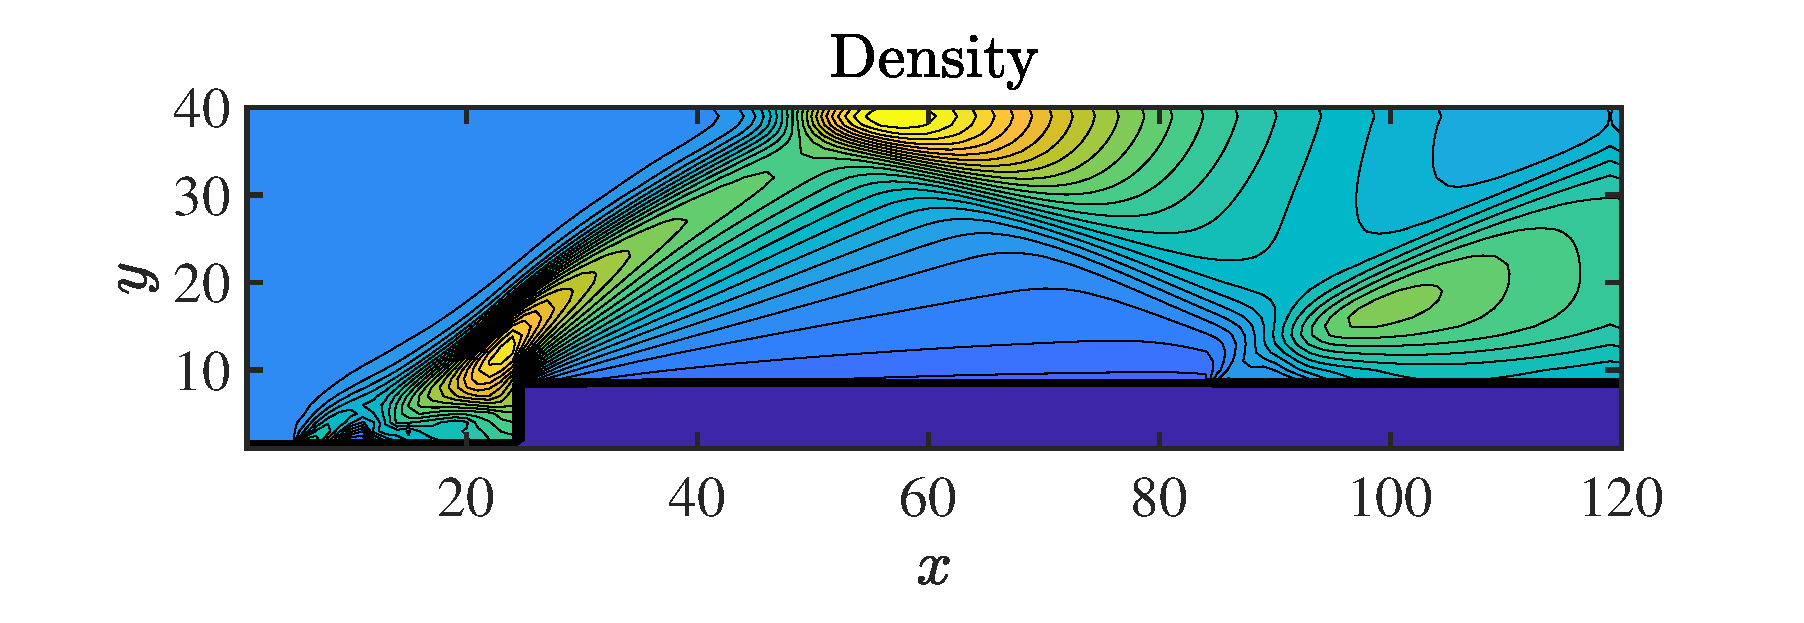
\includegraphics[width=14cm]{density40.eps}
	\caption{密度等线图,网格数是$120\times 40$.}
	\label{fig:density40}
\end{figure}

\begin{figure}[htp]
	\centering
	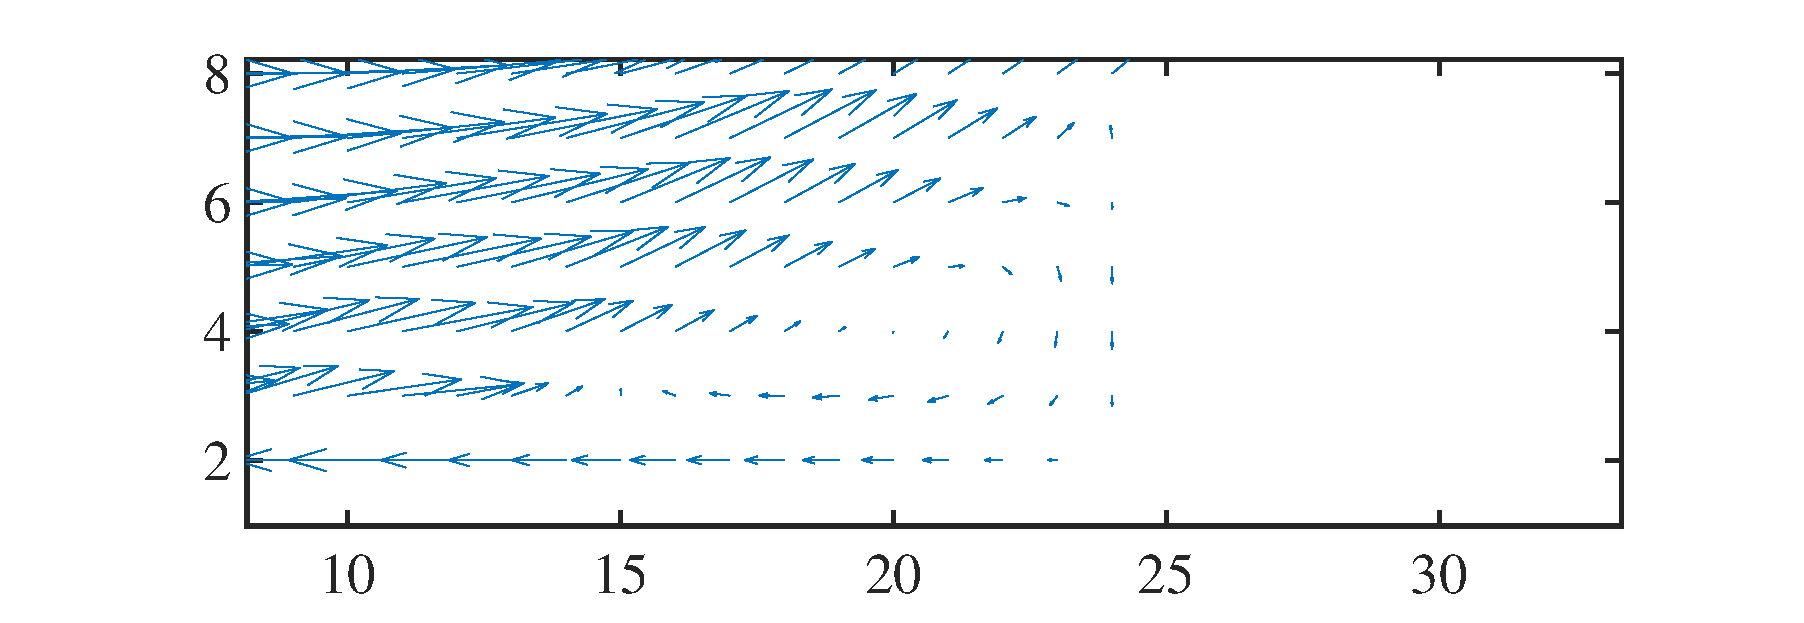
\includegraphics[width=14cm]{eddy.eps}
	\caption{网格数是$120\times 40$时在台阶前形成的流场矢量图。}
	\label{fig:eddy}
\end{figure}




\input{bib.tex}

\end{document}
